\documentclass[10pt,a4paper,fleqn]{report}
\usepackage{amssymb,amsmath,amsthm,amsfonts}
\usepackage{multicol,multirow}
\usepackage{calc}
\usepackage{ifthen}
\usepackage[]{algorithm2e}
\usepackage{graphicx} % for including pictures
\usepackage{subcaption}  % for subfigures
\usepackage{caption}
\usepackage{booktabs} 

\renewcommand{\vec}[1]{\mathbf{#1}}


\begin{document}

\title{Project Work Report \\
	Text Retrieval using Natural Language Processing Methods}
\author{Francesco Carzaniga, 
		Lorenzo Barbera, 
		Qiuhong Lai, 
		Simone Barbaro, 	
		Wenjie He}

\maketitle
\tableofcontents

\chapter*{Abstract}

\chapter{Organization of project}
	\section{Time schedule} 
	
	\section{Objects}
			
		\begin{figure}
			\centering
			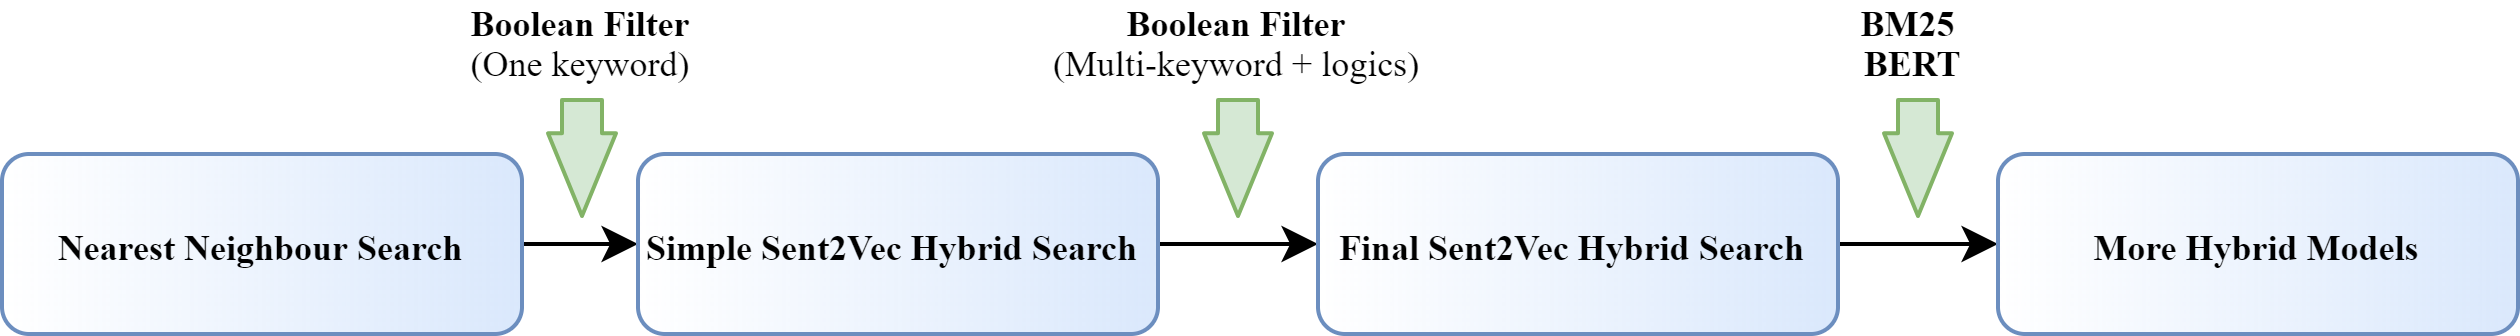
\includegraphics[width=\linewidth]{figure/Object}
			\caption{Project Objects}
			\label{fig:object}
		\end{figure}
			
		The overall goal of the project is to explore natural language processing methods for retrieving scientific content based on a query and potential keywords of interest. We study information retrieval methods and build our search engine step by step. And then we evaluate the performance on a specific dataset.
		We start with basic Sent2Vec + nearest neighbor search. We add keyword Boolean filtering processing into the search engine. And then we consider picking up more than one keywords and using logic strategy to get a subset of corpus so that we have Sent2VecHybrid model. Finally, more hybrid versions of other models are implemented and evaluated.
		
	\section{Task Introduction}	
	
		There are two parts of our project.
		In Part A, we implement and experiment with the methods mentioned above and then evaluate the retrieval performance of various methods on a reduced dataset.
		In part B, we use hybrid search engines we make in part A in more advanced information retrieval tasks. We build a new dataset based on papers from PMC-OA dataset and apply our hybrid search in the dataset. Using M-score, ROUGE score, and DCG score to evaluate and compare the performance of the search engines. Furthermore, some new ranking models are added into our system (like Bert, BertHybrid, FastBM25, etc.).
		
\chapter{Text Retrieval Methods Implementation}			

%	\section{Implementation procedure}

	\begin{figure}[htbp]
		\centering
		\includegraphics[width=\textwidth]{figure/Implementation procedure.png}			
		\caption[]{Text retrieval methods implementation procedure.}
		\label{fig: implementation_procedure}
	\end{figure}
	
	The procedure of text retrieval methods implementation (models) used in this project is shown in figure \ref{fig: implementation_procedure}.
	
	\section{Data Preprocessing}
	Data set is tokenized before fed into the model by filtering out useless characteristics(e.g. out of the set [0-9A-Za-z]), stop-words (e.g.  "a", "the" and so on) and word endings.
	
	\section{Keyword Scorer, Selector and Boolean Filter}
	By computing the term frequency (TF) of each word in the query and the document frequency (IDF) in the corpus, the product of the term frequency and document frequency is the TF-IDF score for each word. 
	
	By determining the number of keywords $N$, the words with top N highest TF-IDF scores are selected for further text retrieving usage.
	
	When multiple keywords are selected, an "or" and "and" logic is applied for the retrieving. 
	The "or" logic can be understood as union of all the articles where the keywords appears.
	The "and" logic can be understood as the intersection of articles lists where each keyword appears (e.g. keyword A appears in article i,j,k and keyword B appears in article i,m,z, the intersection is article i) which can also be understood as selecting the article where all the selected keywords appears.
	
	\section{Ranker / Retrieving Models}
	Several rankers or retrieving methods (models) have been implemented concluding BM25, FastBM25, Sent2Vec, BERT (Bidirectional Encoder Representations from Transformers) and the corresponding hybrid models which combine the existing methods with keyword selection and Boolean filtering.
		
		\subsection{Traditional keyword-based information retrieval methods}		
			\subsubsection{TF-IDF}		
			
				TF-IDF (term frequency-Inverse Document Frequency) is a common weighting technique in information retrieval and data mining. It is often used to mine keywords in the article, and the algorithm is simple and efficient, which is often used by the industry for the initial textual data cleansing. TFIDF reflects how important a word is to a document in a collection or corpus. The TFIDF value increases proportionally to the number of times a word appears in the document and is decreased by the number of documents in the corpus containing the word, which helps to adjust for the fact that some words appear more frequently in general.\\
				
				Term frequency
				$$\operatorname{tf}(t, d)=0.5+0.5 \cdot \frac{f_{t, d}}{\max \left\{f_{t^{\prime}, d}: t^{\prime} \in d\right\}}$$
				where $f_{t,d}$ is the number of times that term $t$ occurs in document $d$. 
				
				Inverse Document Frequency
				$$ idf(t,D) = log \frac{N}{|\{d \in D:T \in d\}|} $$
				where $N$ is total number of documents in the corpus, $|\{d \in D:T \in d\}|$ is number of documents where the term $t$ appears.
					
				Term frequency-Inverse Document Frequency
				$$TFIDF(t,d,D) = tf(t,d) \cdot idf(t,D)$$	

			\subsubsection{BM25}
			
				Okapi BM25 (Best Matching) is a typical algorithm in information retrieval, which is used by search engines to compute the estimated relevance of documents to a given search query. The idea is come up by Stephen E. Robertson, Karen Spärck Jones when they built a probabilistic retrieval framework in the 1970s and 1980s.
				BM25 is a bag-of-words retrieval ranking function which computes the occurrence of query terms in each document and then ranks a set of documents, ignoring their proximity in the document. It is a set of ranking functions with slightly different parameters and components. 
				Given a query $Q$, containing keywords $q_1,...q_n$, the BM25 score of of a document $D$ is:
				$$ score(D,Q) = \sum_{i=1}^{n} IDF(q_i)\cdot \frac{f(q_i,D)\cdot (k_l+1)}{f(q_i,D)+k_l \cdot (1-b+b \cdot \frac{|D|}{avgdl})}$$
				
				where $f(q_i,D)$ is $q_i$'s term frequency in the document D, $|D|$ is the length of the document D in words, and $avgdl$ is the average document length in the text collection from which documents are drawn. $k_l$ and $b$ are free parameters, usually chosen, in absence of an advanced optimization, as $k_l\in [1.2,2.0]$ and $b$ = 0.75. $IDF(q_i)$ is the IDF (inverse document frequency) weight of the query term $q_i$. It is usually computed as:
				$$IDF(q_i)=log \frac{N-n(q_i)+0.5}{n(q_i)+0.5}$$
				
				where N is the total number of documents in the collection, and $n(q_i)$ is the number of documents containing $q_i$.
				
				It can be seen from the formula that BM25 is an improved algorithm based on TFIDF, which adds a constant $k_l$ in TF to limit the growth of TF. BM25 also introduces the concept of average document length, the influence of a single document length on correlation is related to its ratio to the average length.In the TF formula of BM25, two other parameters are introduced: $avgdl$ and $b$. $b$ is a constant, and what it does is it specifies how much $avgdl$ affects the score.
				
			\subsubsection{Fast BM25}
			
				BM25F or Fast-BM25 is an improved algorithm of typical BM25. BM25 considers documents as a whole when calculating relevancy. However, with the development of search technology, documents are gradually replaced by structural data.Such as web pages are likely to be cut into the title, content, subject headings, such as field, the field's contribution to the article topics not same, so the weight needs to be adjusted, BM25 did not consider this, BM25F makes some improvements, in which the document is divided into individual, so BM25F is score in each word in each field of weighted sum.
				
		\subsection{Nearest neighbor search on text embedding}
		
			\subsubsection{Sent2Vec}
			
				Sent2Vec uses a simple but efficient unsupervised objective to train distributed representations of sentences, which allows to compose sentence embeddings using word vectors along with n-gram embeddings, simultaneously training composition and the embedding vectors themselves.
				The model can be seen as a natural extension of the word-contexts from C-BOW model to a large sentence context, with the sentence words being specifically optimized towards additive combination over the sentence, by means of the unsupervised objective function.
				The sentence embedding can be presented as:
				$$ v_s = \frac{1}{|R(S)|} V_{R(S)\sum_{w\in R(S)}v_w} $$
				where $S$ is the sentence, $R(S)$ is the list of n-grams present in $S$, $w$ is every word in the vocabulary, $v_w$ is the word embedding.
				
			
			\subsubsection{BERT - Bidirectional Encoder Representations from Transformers}
			
				Bidirectional Encoder Representations from Transformers (BERT) is a technique developed by Google for Natural Language Processing pre-training. BERT performed well in natural language understanding tasks. BERT originates from pre-training contextual representations including Semi-supervised Sequence Learning, Generative Pre-Training, ELMo, and ULMFit. Different from previous models, BERT is a deeply bidirectional, unsupervised language representation, pre-trained using only a plain text corpus. Context-free models like word2vec or GloVe generate a single word embedding representation for each word in the vocabulary, where BERT takes into account the context for each occurrence of a given word occurring each time.
				
		\subsection{Hybrid search}
				
				A combination of traditional keyword-based methods and text-embedding based methods. 
				A strategy we use in the project is keyword boolean filtering + embedding based ranking.
				
				
	\section{Prediction Evaluation}
	
		Three evaluation methods have been implemented for model's prediction evaluation.
		
		\begin{itemize}
			\item \textbf{"M@L score"} is a score which reveals the percentage of the actual article or "real" article that appears in the first "L" model predictions.
			\item \textbf{ROUGE} (Recall-Oriented Understudy for Gisting Evaluation) is an automatic relevance metrics for searched results evaluation where the similarity between query and searched result is quantitatively computed.
			\item \textbf{NDCG} (Normalized Discounted Cumulative Gain) is a quantitative metrics have been implemented for different retrieval methods evaluation where human rating score and model predicted ranking relationship is quantitatively evaluated.
		\end{itemize}
	
\chapter{Text Retrieval Methods Application}

	\section{Task A: Retrieving abstract using titles}
		\subsection{Task description}
			
			\paragraph{Object}
			In this part, different models are intended to be implemented and evaluated using "M@L score" on the task of retrieving an article abstract given its title in the example dataset.
			
			% dataset and evaluation
			\paragraph{Dataset}
			A reduced dataset which contains 10000 articles concluding the information of doc\_id, doi, year, title, journal name, authors, abstract and full body is used in this part.
			
			% models
			\paragraph{Models (text retrieving methods)}
			In this abstract retrieving using title task, 
			BM25 model, sent2vec model and hybrid search models combining BM25/sent2vec model with keyword Boolean filtering, with different number of keywords and logic filters are implemented.
			
			% predict evaluation
			\paragraph{Evaluation}
			By retrieving abstracts using titles, the performance of implemented models are evaluated using "M@L score" and "ROUGE".
		
		\subsection{Results and evaluation}
			\subsubsection{Retrieving methods comparison}
			
				Model comparisons are made between pure model (e.g. BM25 and Sent2Vec model ) and hybrid models with different filter strategy (e.g. "and" and "or" logic) and different number of keywords by analyzing M@L scores.
				
				% BM25 & hybrid -> fig: hybrid_bm25_and_or
				\begin{figure}[htbp]
					\centering
					\begin{subfigure}[b]{0.48\textwidth}
						\centering
						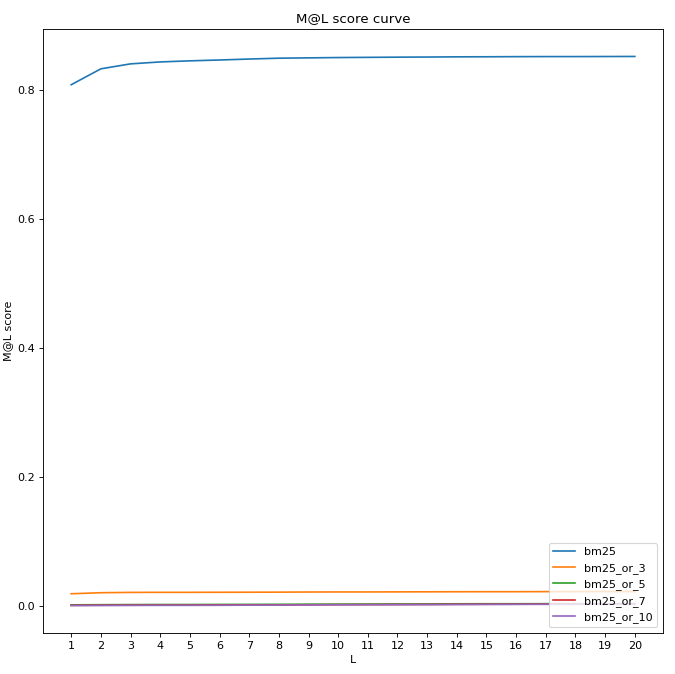
\includegraphics[width=\textwidth]{figure/bm25_or.png}
						\caption{}
						\label{fig: hybrid_bm25_or}
					\end{subfigure}
					\hfill
					\begin{subfigure}[b]{0.48\textwidth}
						\centering
						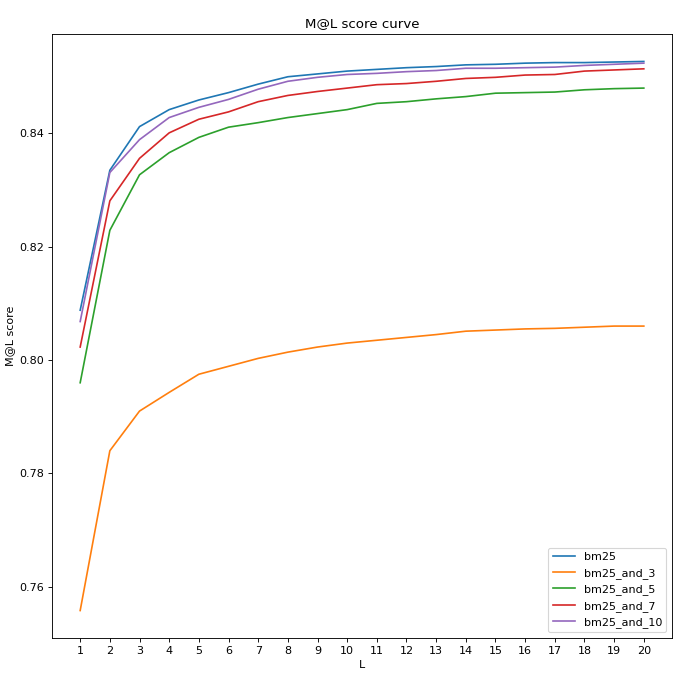
\includegraphics[width=\textwidth]{figure/bm25_and.png}
						\caption{}
						\label{fig: hybrid_bm25_and}
					\end{subfigure}
					\hfill
					\caption[]{Comparison of hybrid search with different filters and different number of keywords for bm25 model. (a) With "or" filter. (b) With "and" filter.}
					\label{fig: hybrid_bm25_and_or}
				\end{figure}
				
				% sent2vec & hybrid
				\begin{figure}[htbp]
					\centering
					\begin{subfigure}[b]{0.48\textwidth}
						\centering
						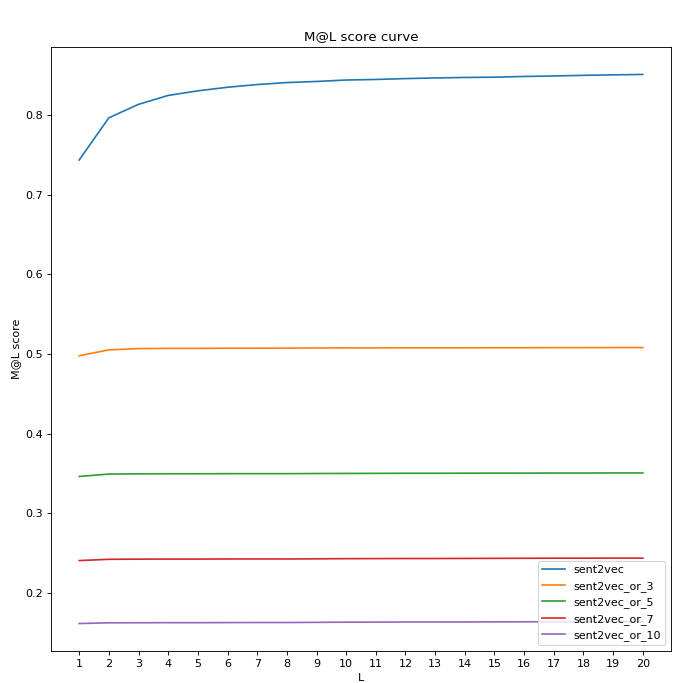
\includegraphics[width=\textwidth]{figure/sent2vec_or.png}
						\caption{}
						\label{fig: hybrid_sent2vec_or}
					\end{subfigure}
					\hfill
					\begin{subfigure}[b]{0.48\textwidth}
						\centering
						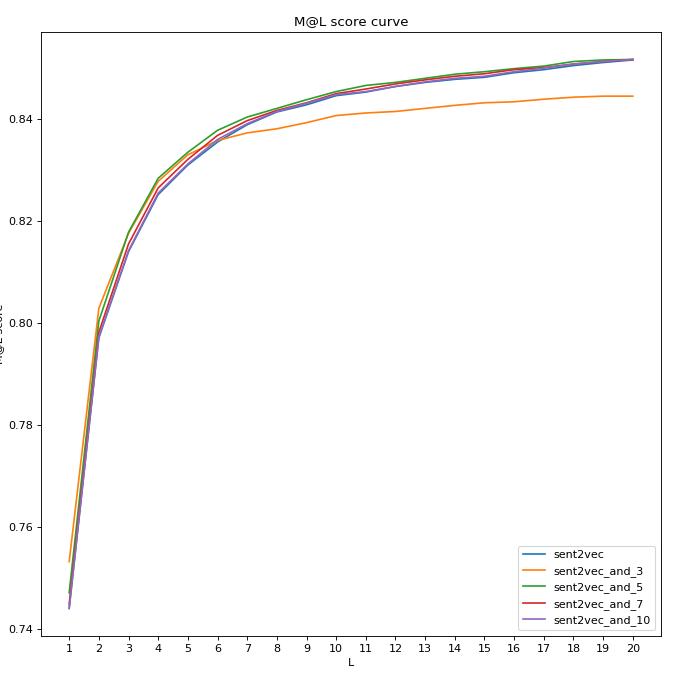
\includegraphics[width=\textwidth]{figure/sent2vec_and.png}
						\caption{}
						\label{fig: hybrid_sent2vec_and}
					\end{subfigure}
					\hfill
					\caption[]{Comparison of hybrid search with different filters and different number of keywords for sent2vec model. (a) With "or" filter. (b) With "and" filter.}
					\label{fig: hybrid_sent2vec_and_or}
				\end{figure}
				
				% model behavior comparisons
				\begin{table}[htbp]
					\centering
					\begin{tabular}{lccccc}
						\toprule
						L     & 1     & 5     & 10    & 15    & 20 \\
						\midrule
						bm25  & 0.8088 & 0.8459 & 0.851 & 0.8522 & 0.8527 \\
						bm25\_and\_10 & 0.8068 & 0.8446 & 0.8504 & 0.8515 & 0.8524 \\
						bm25\_and\_5 & 0.796 & 0.8393 & 0.8442 & 0.8471 & 0.848 \\
						bm25\_and\_3 & 0.7558 & 0.7975 & 0.803 & 0.8053 & 0.806 \\
						sent2vec\_and\_3 & 0.7532 & 0.833 & 0.8407 & 0.8432 & 0.8445 \\
						sent2vec\_and\_5 & 0.7471 & 0.8335 & 0.8454 & 0.8493 & 0.8517 \\
						sent2vec\_and\_10 & 0.7441 & 0.8312 & 0.8448 & 0.8484 & 0.8517 \\
						sent2vec & 0.744 & 0.831 & 0.8446 & 0.8482 & 0.8516 \\
						sent2vec\_or\_3 & 0.4978 & 0.5071 & 0.5077 & 0.5079 & 0.5081 \\
						sent2vec\_or\_5 & 0.346 & 0.3494 & 0.3498 & 0.3502 & 0.3504 \\
						sent2vec\_or\_10 & 0.161 & 0.1621 & 0.1627 & 0.1631 & 0.1634 \\
						bm25\_or\_3 & 0.0189 & 0.0211 & 0.0217 & 0.0221 & 0.0223 \\
						bm25\_or\_5 & 0.0017 & 0.0022 & 0.0028 & 0.0034 & 0.0036 \\
						bm25\_or\_10 & 0.0006 & 0.0009 & 0.0017 & 0.0023 & 0.0026 \\
						\bottomrule
					\end{tabular}%
					\caption{Comparison of M@L score for all tests in tabular form}
					\label{tab: comparison of ml scores of all models}%
				\end{table}%
				
				
				The comparison of BM25 model and BM25 hybrid models with \textbf{"or" filter} M@L scores can be seen from the figure \ref{fig: hybrid_bm25_or} and the comparison of BM25 model and BM25 hybrid models with \textbf{"and" filter} M@L scores can be seen from the figure \ref{fig: hybrid_bm25_or}.
				The comparison between "or" and "and" models is shown in figure \ref{fig: hybrid_bm25_and_or}.
				Similarly, the model comparison of Sent2Vec models is shown in figure \ref{fig: hybrid_sent2vec_and_or}.			
				The full comparison data is shown in table \ref{tab: comparison of ml scores of all models}.
				
				\paragraph{Comparison of pure models and hybrid models with different number of keywords}
				The BM25 model and Sent2Vec model is named as "pure model" here.
				
				
				\subparagraph{Application of keyword filtering}
				As shown in the figure \ref{fig: hybrid_bm25_or} and figure \ref{fig: hybrid_bm25_and}, the M@L score of hybrid BM25 models are lower than standard BM25 model.
				Similar tendency is discovered in Sent2Vec models as shown in figure \ref{fig: hybrid_sent2vec_and_or}.
				However, the M@L score differences between pure model and hybrid models are much less in Sent2Vec model than BM25 model and even in Sent2Vec model, the M@L score is improved for small L which means that the filter helps this model reduce the amount of false positives.\\
				
				It indicates that adding keyword filtering into the retrieval models could be more efficient improving the performance of Sent2Vec model than BM25 model.
				
				\subparagraph{Number of keywords}
				As shown in figure \ref{fig: hybrid_bm25_and}, a higher number of keyword tends to lead to a relatively higher M@L score in the hybrid BM25 model with "and" logic. 10 keyword selection would lead to a similar behavior compared with BM25 model. However, the behavior of keyword number seems to be opposite in the hybrid BM25 model with "or" logic as shown in figure \ref{fig: hybrid_bm25_or}  where a higher number of keywords would lead to a lower model performance.
				Similar tendencies are also found in Sent2Vec models as shown in figure \ref{fig: hybrid_sent2vec_and_or}.
				
				It indicates that a higher number of keywords would help improve the M@L score in hybrid models with a "and" logic filter and in contrast, fewer keywords would help improve the M@L score in hybrid models with a "or" logic filter.
				
				This makes sense since with an "and" logic filter, a higher number of keywords would lead to a higher restriction which means higher correlation and is tend to find the precise content and therefore a better M@L score.
				
				\paragraph{Comparison of "and" and "or" filter logic}
				By comparing the hybrid BM25 models with "or" and "and" logic as shown in 
				figure \ref{fig: hybrid_bm25_or} and figure \ref{fig: hybrid_bm25_and} respectively. It can be found that the "and" logic will lead to much higher M@L score compared with "or" logic and "and" logic will lead to a similar M@L score tendency when increasing $L$ value. Similar behavior is also discovered by comparing the hybrid Sent2Vec models.
				
				It shows that in the task of retrieving abstract using title, hybrid models's "and" logic can be a better option compared with the "or" logic.
				
				\paragraph{Comparison of BM25 model and Sent2Vec model}
				By comparing the performance of BM25 model and Sent2Vec pure model as shown in figure \ref{fig: hybrid_bm25_and_or} and figure \ref{fig: hybrid_sent2vec_and_or}, it is found that BM25 model has a higher M@L score than Sent2Vec model with the $L$ value ranging from 1 to 20.				
				However, it is also find that the Sent2Vec model increases much faster than BM25 do which might lead to a higher value when $L$ is bigger than 20.
				
				But it is known that a higher M@L value with a lower $L$ value indicates a more precise prediction. 
				So it can be concluded that in the task of retrieving abstract using title, the BM25 model has a better prediction than Sent2Vec model.
			\subsubsection{Metrics Comparison}
				\paragraph{M@L score}
					
					% BM25
					\begin{figure}[htbp]
						\centering
						\begin{subfigure}[b]{0.48\textwidth}
							\centering
							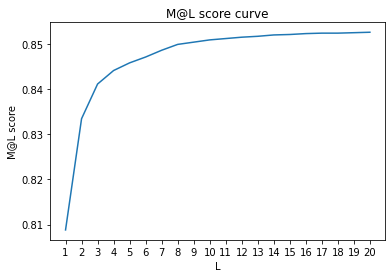
\includegraphics[width=\textwidth]{figure/partA_bm25_ml_score.png}
							\caption{}
							\label{fig: bm25_mlscore}
						\end{subfigure}
						\hfill
						\begin{subfigure}[b]{0.48\textwidth}
							\centering
							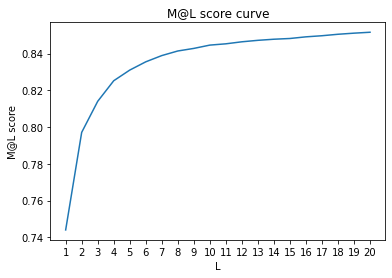
\includegraphics[width=\textwidth]{figure/partA_sent2vec_ml_score.png}
							\caption{}
							\label{fig: sent2vec_mlscore}
						\end{subfigure}
						\hfill
						\begin{subfigure}[b]{0.48\textwidth}
							\centering
							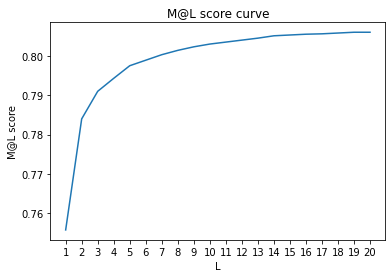
\includegraphics[width=\textwidth]{figure/partA_Bm25HybridRanker_ml_score.png}
							\caption{}
							\label{fig: Bm25HybridRanker_mlscore}
						\end{subfigure}
						\hfill
						\begin{subfigure}[b]{0.48\textwidth}
							\centering
							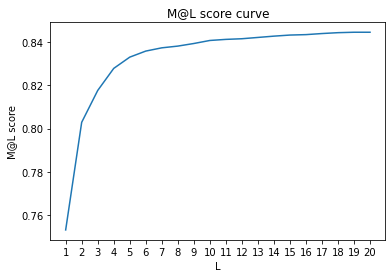
\includegraphics[width=\textwidth]{figure/partA_Sent2VecHybridRanker_ml_score.png}
							\caption{}
							\label{fig: Sent2VecHybridRanker_mlscore}
						\end{subfigure}
						\hfill
						\caption[]{Model retrieving performance - M@L score. (a)BM25. (b)Sent2Vec. (c)BM25 Hybrid model  ("and" logic and 3 keywords). (d)Sent2Vec Hybrid model ("and" logic and 3 keywords). }
						\label{fig: }
					\end{figure}
					
					% Table generated by Excel2LaTeX from sheet 'M@L score'
					\begin{table}[htbp]
						\centering
						\caption{Add caption}
						\begin{tabular}{lcc}
							\toprule
							models & M@1   & M@20 \\
							\midrule
							BM25  & 0.8088 & 0.8527 \\
							BM25\_and\_3 & 0.7558 & 0.806 \\
							Sent2Vec & 0.744 & 0.8516 \\
							sent2vec\_and\_3 & 0.7532 & 0.8445 \\
							\bottomrule
						\end{tabular}%
						\caption{M@L scores of different text retrieval models in task A.}
						\label{tab: models_ml_scores}%
					\end{table}%
										
					
					\textbf{BM25} 
					model behavior concluding the M@L score is shown in figure \ref{fig: bm25_mlscore} with a M@1 score of 0.8088 and a M@20 score of 0.8527.
					
					\textbf{Sent2Vec} 
					model behavior concluding the M@L score is shown in figure \ref{fig: sent2vec_mlscore} with a M@1 score of 0.7558 and a M@20 score of 0.806.
					
					\textbf{BM25 hybrid search ("and" logic and 3 keywords)} 
					model behavior concluding the M@L score is shown in figure \ref{fig: Bm25HybridRanker_mlscore} with a M@1 score of 0.744 and a M@20 score of 0.8516.
					
					\textbf{Sent2Vec hybrid search ("and" logic and 3 keywords)} 
					model behavior concluding the M@L score is shown in figure \ref{fig: Sent2VecHybridRanker_mlscore} with a M@1 score of 0.7532 and a M@20 score of 0.8445.
					
					The M@1 score and M@20 score of these models are gathered in the table \ref{tab: models_ml_scores}.
					
					It can be concluded that, a higher M@L score is going to be obtained with a higher $L$ value. There is an obvious M@L score increase with a $L$ value increasing from 1 to 5, and it tends to saturate with a $ L $ value approaching 10.
					
					It seems a $L$ value of 20 can be enough and efficient for revealing the quality of retrieving method which can also be understand as model predicted first 20 articles would be efficient to reveal the model's retrieving ability.
					
					In addition, picking a suitable $L$ value for evaluation should be considered only when there is a requirement or limitation for the computation time and computation memory. 
					
					Further comparisons between different retrieving models would be discussed in the following sections.
				
				\paragraph{ROUGE score (Recall-Oriented Understudy for Gisting Evaluation) }
				
					\begin{table}[htbp]
						\centering
						\begin{tabular}{crrrr}
							\toprule
							\multirow{4}[2]{*}{bm25} & \multicolumn{1}{l}{rouge-1:} & \multicolumn{1}{l}{P: 32.84} & \multicolumn{1}{l}{R: 41.65} & \multicolumn{1}{l}{F1: 36.72} \\
							& \multicolumn{1}{l}{rouge-2:} & \multicolumn{1}{l}{P: 9.51} & \multicolumn{1}{l}{R: 12.07} & \multicolumn{1}{l}{F1: 10.64} \\
							& \multicolumn{1}{l}{rouge-l:} & \multicolumn{1}{l}{P: 18.33} & \multicolumn{1}{l}{R: 23.25} & \multicolumn{1}{l}{F1: 20.5} \\
							& \multicolumn{1}{l}{rouge-w:} & \multicolumn{1}{l}{P: 18.33} & \multicolumn{1}{l}{R: 23.25} & \multicolumn{1}{l}{F1: 20.5} \\
							\midrule
							\multirow{4}[2]{*}{bm25\_and\_3} & \multicolumn{1}{l}{rouge-1:} & \multicolumn{1}{l}{P: 32.36} & \multicolumn{1}{l}{R: 38.48} & \multicolumn{1}{l}{F1: 35.16} \\
							& \multicolumn{1}{l}{rouge-2:} & \multicolumn{1}{l}{P: 9.37} & \multicolumn{1}{l}{R: 11.15} & \multicolumn{1}{l}{F1: 10.18} \\
							& \multicolumn{1}{l}{rouge-l:} & \multicolumn{1}{l}{P: 18.73} & \multicolumn{1}{l}{R: 22.27} & \multicolumn{1}{l}{F1: 20.34} \\
							& \multicolumn{1}{l}{rouge-w:} & \multicolumn{1}{l}{P: 18.73} & \multicolumn{1}{l}{R: 22.27} & \multicolumn{1}{l}{F1: 20.34} \\
							\midrule
							\multirow{4}[2]{*}{sent2vec} & \multicolumn{1}{l}{rouge-1:} & \multicolumn{1}{l}{P: 33.53} & \multicolumn{1}{l}{R: 41.41} & \multicolumn{1}{l}{F1: 37.05} \\
							& \multicolumn{1}{l}{rouge-2:} & \multicolumn{1}{l}{P: 9.68} & \multicolumn{1}{l}{R: 11.96} & \multicolumn{1}{l}{F1: 10.7} \\
							& \multicolumn{1}{l}{rouge-l:} & \multicolumn{1}{l}{P: 18.71} & \multicolumn{1}{l}{R: 23.11} & \multicolumn{1}{l}{F1: 20.68} \\
							& \multicolumn{1}{l}{rouge-w:} & \multicolumn{1}{l}{P: 18.71} & \multicolumn{1}{l}{R: 23.11} & \multicolumn{1}{l}{F1: 20.68} \\
							\midrule
							\multirow{4}[2]{*}{sent2vec\_and\_3} & \multicolumn{1}{l}{rouge-1:} & \multicolumn{1}{l}{P: 31.9} & \multicolumn{1}{l}{R: 38.7} & \multicolumn{1}{l}{F1: 34.98} \\
							& \multicolumn{1}{l}{rouge-2:} & \multicolumn{1}{l}{P: 9.22} & \multicolumn{1}{l}{R: 11.19} & \multicolumn{1}{l}{F1: 10.11} \\
							& \multicolumn{1}{l}{rouge-l:} & \multicolumn{1}{l}{P: 18.51} & \multicolumn{1}{l}{R: 22.46} & \multicolumn{1}{l}{F1: 20.3} \\
							& \multicolumn{1}{l}{rouge-w:} & \multicolumn{1}{l}{P: 18.51} & \multicolumn{1}{l}{R: 22.46} & \multicolumn{1}{l}{F1: 20.3} \\
							\midrule
							&       &       &       &  \\
						\end{tabular}%
						\caption{Rouge score calculated for different retrieving models}
						\label{tab: rouge_score}%					
					\end{table}%
					
					The calculated ROUGE score is shown in table \ref{tab: rouge_score} which can also be a reference evaluating the performance of retrieving models.	As "P" indicates precision and "R" indicates recall and "F1" is the multiplication-kind operation of "P" and "R", therefore for simplification, ROUGE F1 scores are selected for further analysis.
					
					A higher ROUGE "F1" value indicates that the model generates a better prediction (predicts more accurate article) compared with the standard reference articles.
					
					It can be found that the ROUGE-1 value is 2-3 times higher than ROUGE-2, ROUGE-L has same value as ROUGE-W and ROUGE-L value is lower than ROUGE-1 value and higher than ROUGE-2 value. 
					
					Because of the more restricted ROUGE-2 condition where 2-gram between two string list should correlate and in comparison ROUGE-1 only need 1-gram to be correlated, the ROUGE-1 is much higher than ROUGE-2 value.					
					Since ROUGE-L "L" indicates the longest common subsequent, it make sense it has a lower value than ROUGE-1 and higher value than ROUGE-2.					
					ROUGE-W is the modification of ROUGE-L, which considers the embedding sequences. Considering our task, it is hard to find the absolute same sequence as title from abstract, so the embedding sequences won't effect the result and it make sense that the ROUGE-W have same value as ROUGE-L.
						
				\paragraph{Evaluation metrics comparison}

					\begin{figure}
						\centering
						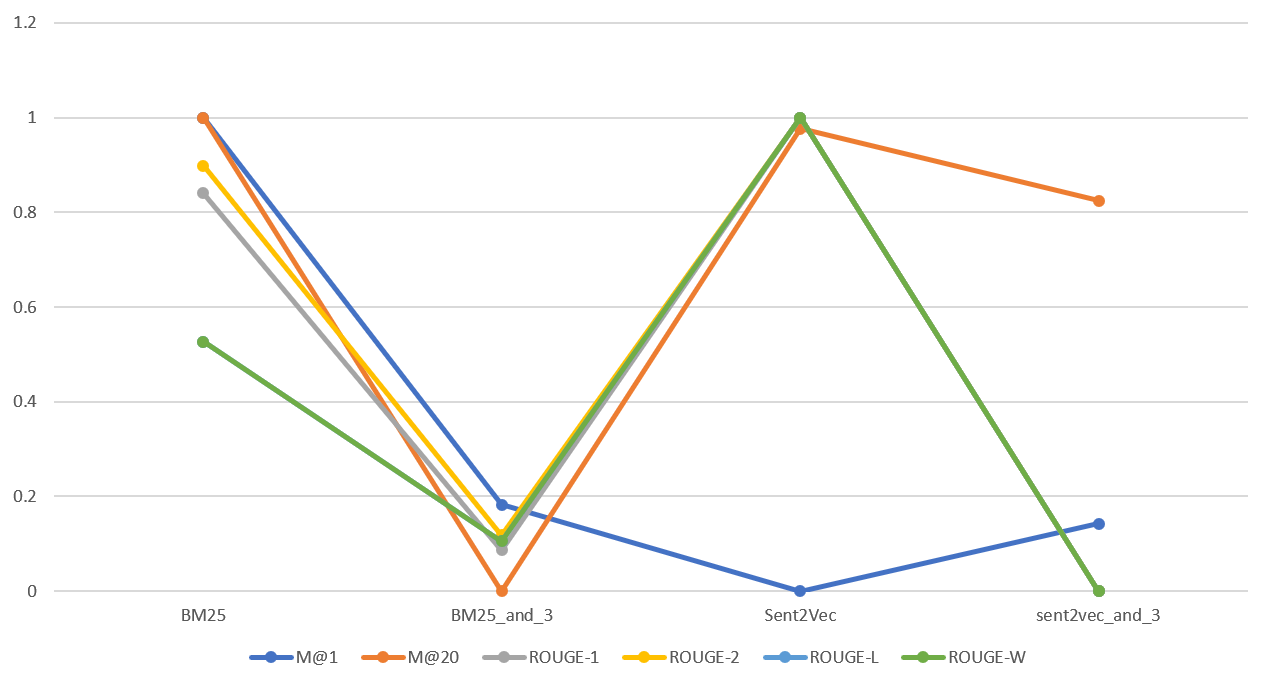
\includegraphics[width=0.9\linewidth]{figure/partA_normalized_evaluation_metrics}
						\caption{Normalized scores of different evaluation matrices using different models.}
						\label{fig: partanormalizedevaluationmetrics}
					\end{figure}
				
					To compare the different evaluation metrics, the scores are normalized to [0-1] for further analysis as shown in figure \ref{fig: partanormalizedevaluationmetrics}.
					
					From this graph, it can be found that M@20, ROUGE-1 and ROUGE-2 have correlated tendency which can help reveal the performance of different models. However, M@1, ROUGE-L and ROUGE-W seem to have different tendency than normal tendency.
					
					It can also be concluded from this normalized figure that the addition of keyword filtering function (hybrid model) in this task doesn't improve the text retrieving performance (prediction). BM25 model seems to have similar performance to Sent2Vec model and has a better performance than other hybrid models.
					
			
		\subsection{Conclusion}	
			
			\paragraph{Retrieval methods}
			
				In general, BM25 model seems to have similar performance to Sent2Vec model and has a better performance than other hybrid models.
				It might be because of the nature of the task, since title and abstract are much shorted than the body of the abstracts. 
				
			\paragraph{Hybrid tuning methods}
				
				In this specific task, adding keyword filtering seems (applying hybrid model) to have the potential to improve the Sent2Vec model performance but not for BM25 model.
				
				Hybrid models with \textbf{"and" logic} performs much better than models with \textbf{"or" logic}.
				
				A \textbf{higher number of keywords} in "and" logic and a lower number of keywords in "or" logic would help improve the performance of hybrid models.
			
			\paragraph{Evaluation metrics}
				
				In this task, it is found that M@20, ROUGE-1 and ROUGE-2 metrics have similar tendency revealing the performance of text retrieving method which is supposed to be better than other metrics like M@1, ROUGE-L and ROUGE-W. 
				
				The normalized scores method can also be used for evaluating the performance in other tasks.
		
	\newpage
	\section{Task B: Retrieving discussions using results}

	In the second task, the developed hybrid search engines are applied in more advanced information retrieval tasks.
	A new human rated result-and-discussion-pairs dataset based on papers from PMC-OA dataset are created for 10 different topics.
	The developed search engines (some new ranking models are added like Bert, BertHybrid, FastBM25, etc.) with different keyword selector methods (SentenceTokenizer,  PuctDigitRemoveTokenizer, split) are used to 
	firstly pair result paragraphs to discussion paragraphs ("Pairing Task"), 
	then retrieve discussion paragraphs with given result paragraph ("Retrieval Task").
	The performance of the search engines are evaluate and compard using M@L-score, ROUGE score, and NDCG score.
	
	\subsection{Task Procedure}
		
		\begin{figure}[htbp]
			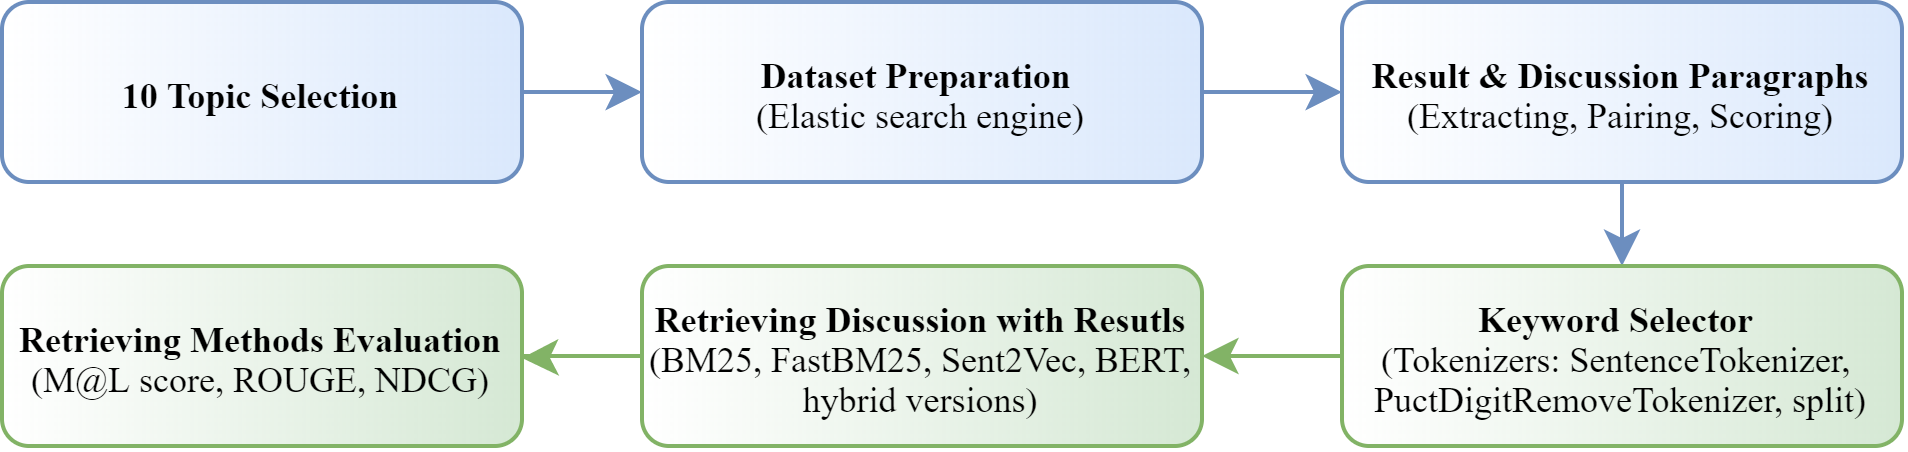
\includegraphics[width=\textwidth]{figure/taskB_procedure.png}
			\caption[]{Result and discussion pairing task processing procedures.}
			\label{fig: taskB_procedure}
		\end{figure}
	
		As shown in figure \ref{fig: taskB_procedure}, the second task is divided into following major procedures:
		
		\paragraph{Topic Selection:}
		
			10 different topics are chosen for article selection in this task. The words from table S1 in the document "Inheritance patterns in citation networks reveal scientific memes – supplementary material" is used as a reference for the topic selection.
			
			% todo add topics
			The chosen topics concluding: Reinforcement Learning, Auditory Learning, Bluetongue, Meliodosis, Malaria, West Nile virus, cerebrospinal venous, Buruli ulcer
			
		\paragraph{Dataset Preparation:}
		
			For each topic, Elastic search engine is used to get 1 paper and then 9 most similar papers from PMC-OA dataset is retrieved. In total there are 100 original papers to work on.
			
		\paragraph{Result and Discussion Paragraphs Processing and Scoring:}
			
			With the full body extracted from the 100 papers, the result and discussion paragraphs are further extracted from the full body.
			The relevant results and discussions are paired and further human scored in the range of [0,1,2,3,4] according to the degree of correlation in between with a score of 0 indicating no relation between selected result paragraph and with a score of 4 indicating the discussion paragraph is exactly talking about the result paragraph.	
			Finally 2547 human rated scores are generated for result and discussion pairs.
			Detailed data structure and the code modules would be introduced in Appendix \ref{sk: dataandcode}.
		
		\paragraph{Keyword Selector:}
			
			To select the keywords for the retrieving task, different tokenizors are implemented concluding SentenceTokenizor, PuctDigitRemoveTokenizor and simple split function.
		
		\paragraph{Pairing and Retrieving Discussion with Results:}
			
			Task B is divided into to tasks, first "Pairing Task": the discussion paragraphs are paired with given result paragraphs then the retrieval methods (BM25, FastBM25, Sent2Vec, BERT and their hybrid versions) are evaluated according to M@L scores.
			
			Second, "Retrieval Task": by giving a human rating score {0,1,2,3,4} to each retrieved search result according to its relevance to the query, different methods are evaluated by using ROUGE and NDCG quantitative matrices.
		
		\paragraph{Retrieving Methods Evaluation:}
			
			The search results of different models (model predictions) are evaluated together with human rated scores using M@L score, ROUGE and NDCG in this task.
	

	\subsection{Results and evaluation}			
		
		\subsubsection{Pairing Task} % M@L
			
			In the pairing task, different models are applied concluding BM25, FastBM25, Sent2Vec, BERT and their hybrid versions.
			The discussion paragraphs are paired with result paragraphs, the M@L metrics is used for retrieving method and hybrid effect analysis.
			
			The retrieving performance of different models is shown in the figure \ref{fig: pairingtaskmlscore}. As can be seen from the figure, the values tend to become same (0.96) when L increases from 1 to 20.
			
			\paragraph{Retrieval methods} % BM25
				According to the M@L absolute values, the models' performance are divided into 3 categories: "high M@L score", "middle M@L score" and "low M@L score" as listed in the table \ref{tab: pairingcategorization}.
				
				From this categorization, it can be find that in pairing task, BM25 and FastBM25 retrieving methods are categorized as "high M@L values" and indeed have better performance compared with other methods. It can be concluded that BM25 and FastBM25 have better performance than other methods in pairing task.
				In addition, hybrid version of BM25 and FastBM25 models have lower M@L values which means 
				the application of hybrid functions to BM25 and FastBM25 models would lead to reduced performance.
				
				% todo update sent2vec model results into figures
				\begin{figure}[htbp]
					\centering
					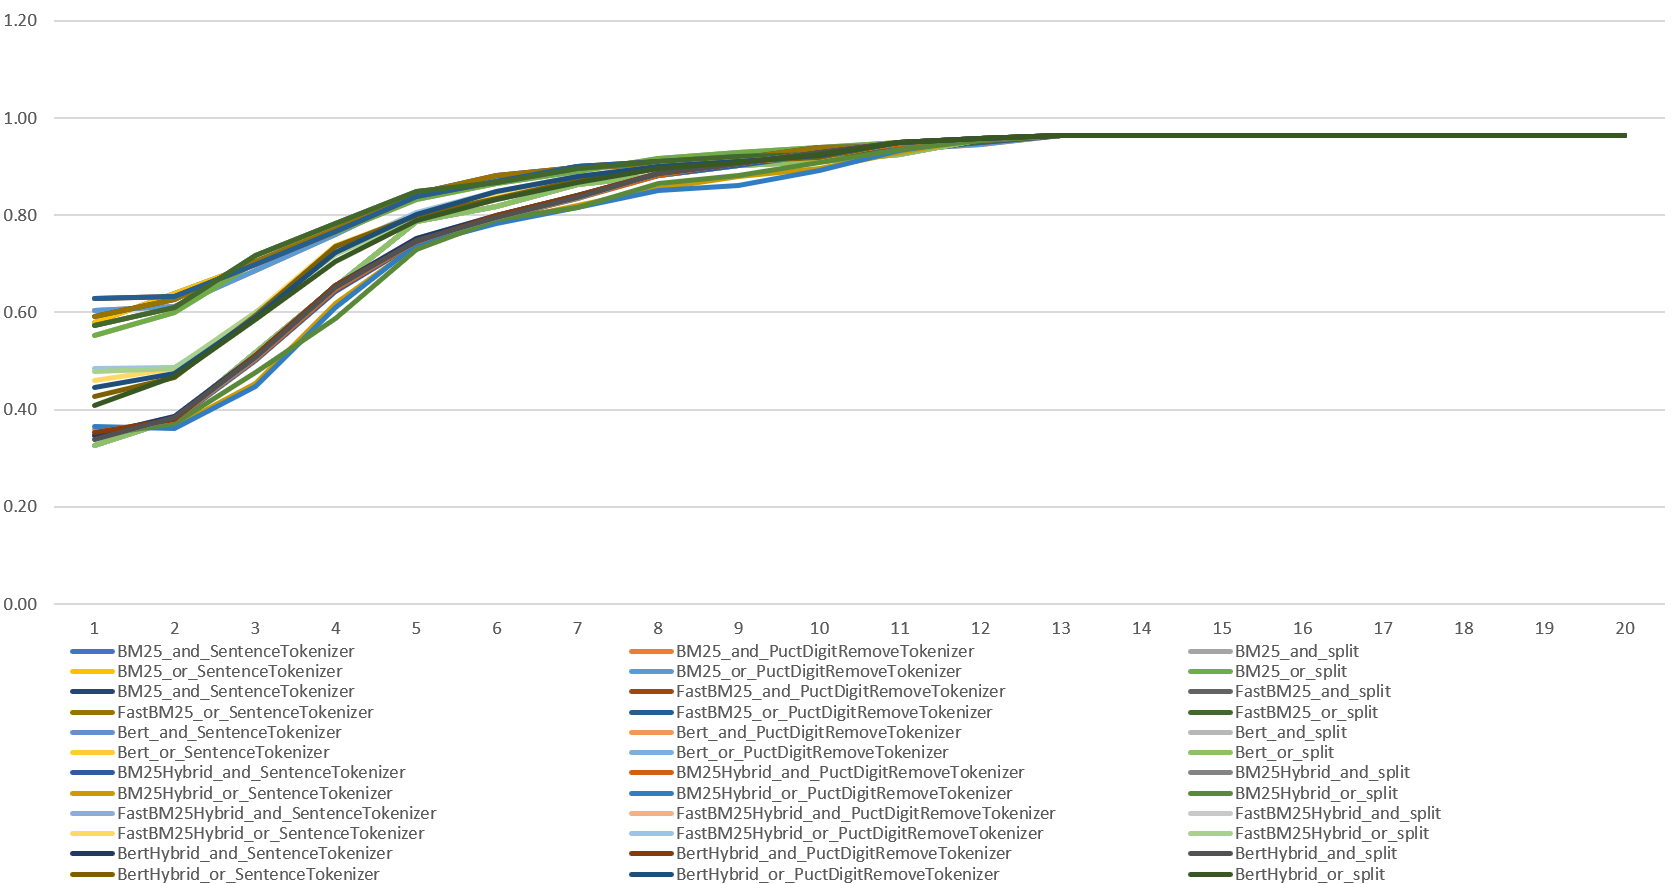
\includegraphics[width=\textwidth]{figure/partB_pairing_M@L_all_models.png}
					\caption[]{Pairing task's M@L score of all the models.}
					\label{fig: pairingtaskmlscore}
				\end{figure}
				
				\begin{table}[htbp]
					\centering
					\resizebox{\textwidth}{!}{
						\begin{tabular}{rrrr}
							\toprule
							\multicolumn{1}{c}{\multirow{12}[2]{*}{high M@L score}} & \multicolumn{1}{l}{BM25\_and\_SentenceTokenizer} & \multicolumn{1}{c}{\multirow{18}[4]{*}{low M@L score}} & \multicolumn{1}{l}{Bert\_and\_SentenceTokenizer} \\
							& \multicolumn{1}{l}{BM25\_and\_PuctDigitRemoveTokenizer} &       & \multicolumn{1}{l}{Bert\_and\_PuctDigitRemoveTokenizer} \\
							& \multicolumn{1}{l}{BM25\_and\_split} &       & \multicolumn{1}{l}{Bert\_and\_split} \\
							& \multicolumn{1}{l}{BM25\_or\_SentenceTokenizer} &       & \multicolumn{1}{l}{Bert\_or\_SentenceTokenizer} \\
							& \multicolumn{1}{l}{BM25\_or\_PuctDigitRemoveTokenizer} &       & \multicolumn{1}{l}{Bert\_or\_PuctDigitRemoveTokenizer} \\
							& \multicolumn{1}{l}{BM25\_or\_split} &       & \multicolumn{1}{l}{Bert\_or\_split} \\
							& \multicolumn{1}{l}{FastBM25\_and\_SentenceTokenizer} &       & \multicolumn{1}{l}{BM25Hybrid\_and\_SentenceTokenizer} \\
							& \multicolumn{1}{l}{FastBM25\_and\_PuctDigitRemoveTokenizer} &       & \multicolumn{1}{l}{BM25Hybrid\_and\_PuctDigitRemoveTokenizer} \\
							& \multicolumn{1}{l}{FastBM25\_and\_split} &       & \multicolumn{1}{l}{BM25Hybrid\_and\_split} \\
							& \multicolumn{1}{l}{FastBM25\_or\_SentenceTokenizer} &       & \multicolumn{1}{l}{BM25Hybrid\_or\_SentenceTokenizer} \\
							& \multicolumn{1}{l}{FastBM25\_or\_PuctDigitRemoveTokenizer} &       & \multicolumn{1}{l}{BM25Hybrid\_or\_PuctDigitRemoveTokenizer} \\
							& \multicolumn{1}{l}{FastBM25\_or\_split} &       & \multicolumn{1}{l}{BM25Hybrid\_or\_split} \\
							\cmidrule{1-2}    \multicolumn{1}{c}{\multirow{6}[2]{*}{middle M@L score}} & \multicolumn{1}{l}{BertHybrid\_or\_SentenceTokenizer} &       & \multicolumn{1}{l}{FastBM25Hybrid\_and\_SentenceTokenizer} \\
							& \multicolumn{1}{l}{BertHybrid\_or\_PuctDigitRemoveTokenizer} &       & \multicolumn{1}{l}{FastBM25Hybrid\_and\_PuctDigitRemoveTokenizer} \\
							& \multicolumn{1}{l}{BertHybrid\_or\_split} &       & \multicolumn{1}{l}{FastBM25Hybrid\_and\_split} \\
							& \multicolumn{1}{l}{FastBM25Hybrid\_or\_SentenceTokenizer} &       & \multicolumn{1}{l}{BertHybrid\_and\_SentenceTokenizer} \\
							& \multicolumn{1}{l}{FastBM25Hybrid\_or\_PuctDigitRemoveTokenizer} &       & \multicolumn{1}{l}{BertHybrid\_and\_PuctDigitRemoveTokenizer} \\
							& \multicolumn{1}{l}{FastBM25Hybrid\_or\_split} &       & \multicolumn{1}{l}{BertHybrid\_and\_split} \\
							\midrule
							&       &       &  \\
						\end{tabular}}
					\caption{Pairing models categorization according to M@L scores.}
					\label{tab: pairingcategorization}%
				\end{table}%
								
				\begin{figure}[htbp]
					\centering
					\begin{subfigure}[b]{0.8\textwidth}
						\centering
						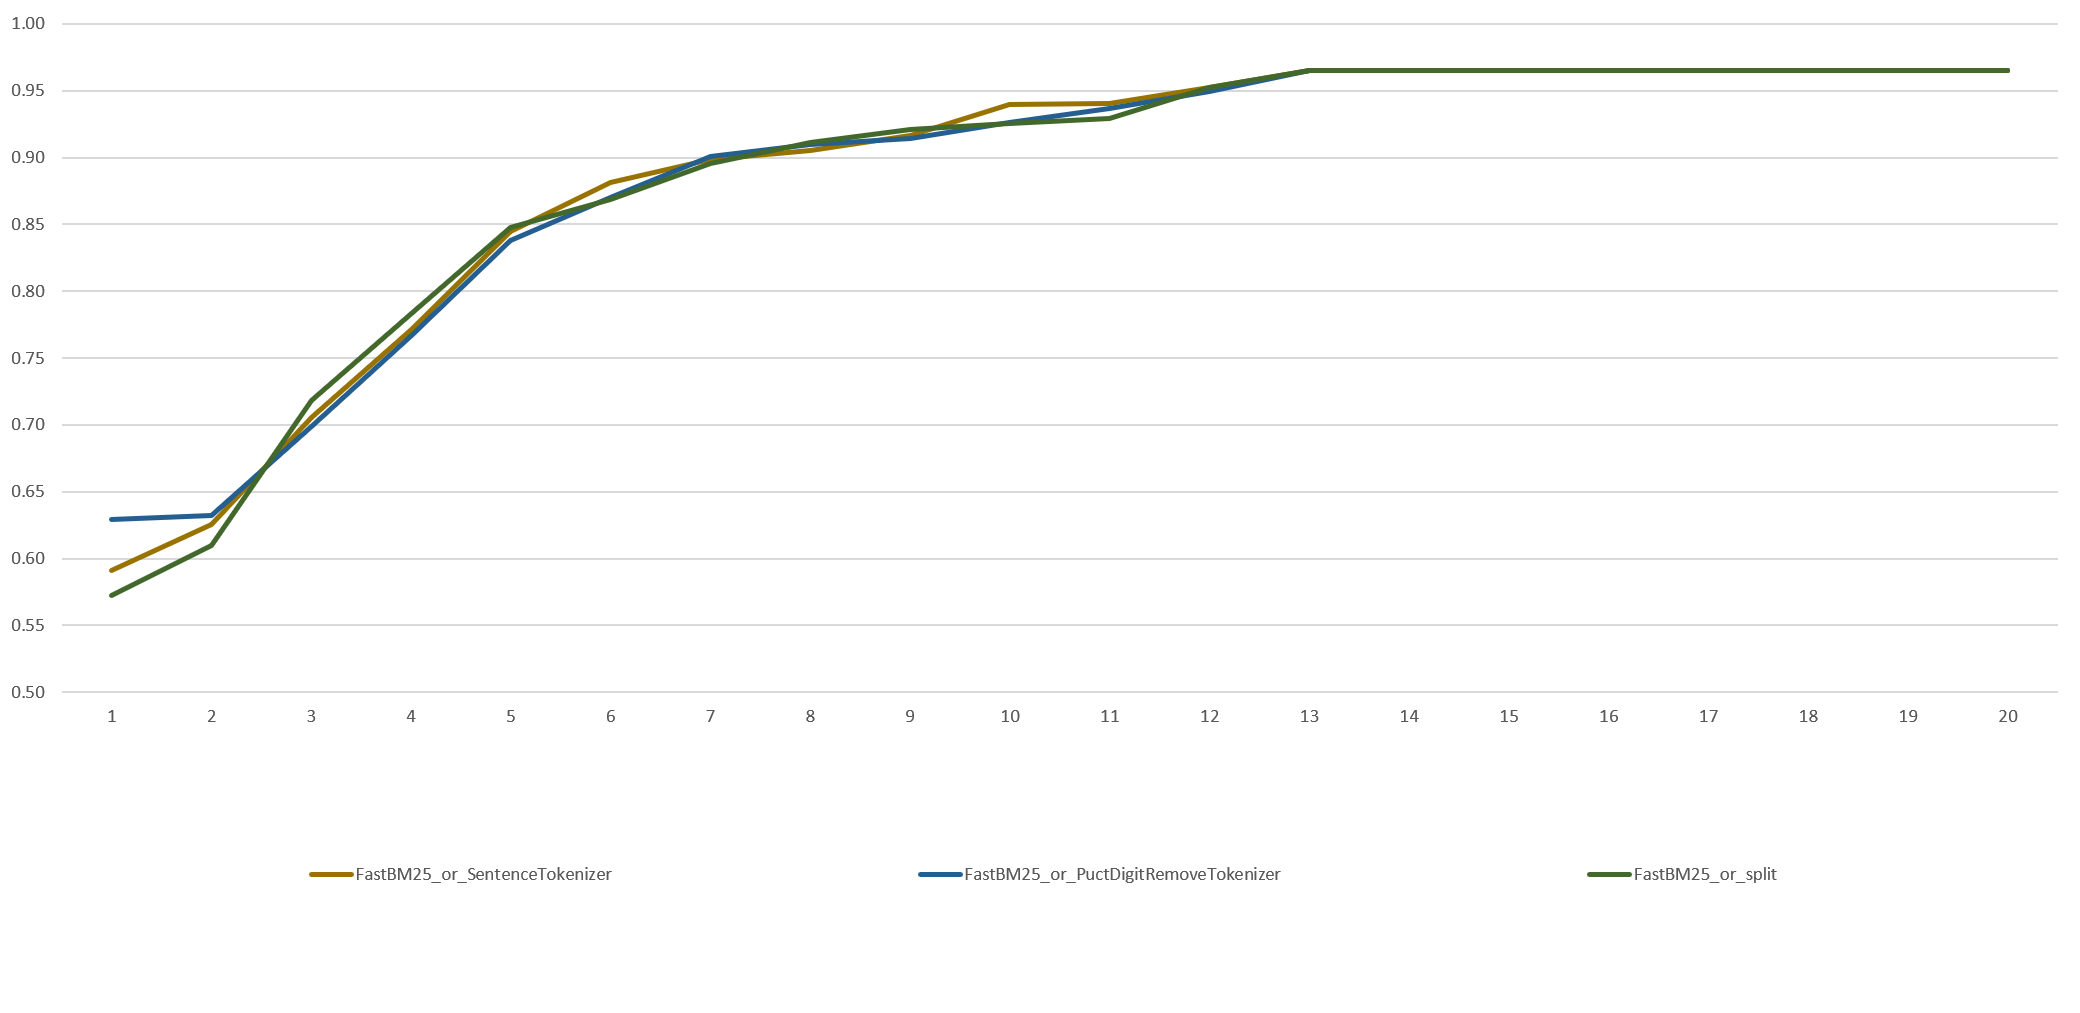
\includegraphics[width=\textwidth]{figure/partB_pairing_tokenizor_or.png}
						\caption{}
						\label{fig: pairingtokenizoreffect_or}
					\end{subfigure}
					\hfill
					\begin{subfigure}[b]{0.8\textwidth}
						\centering
						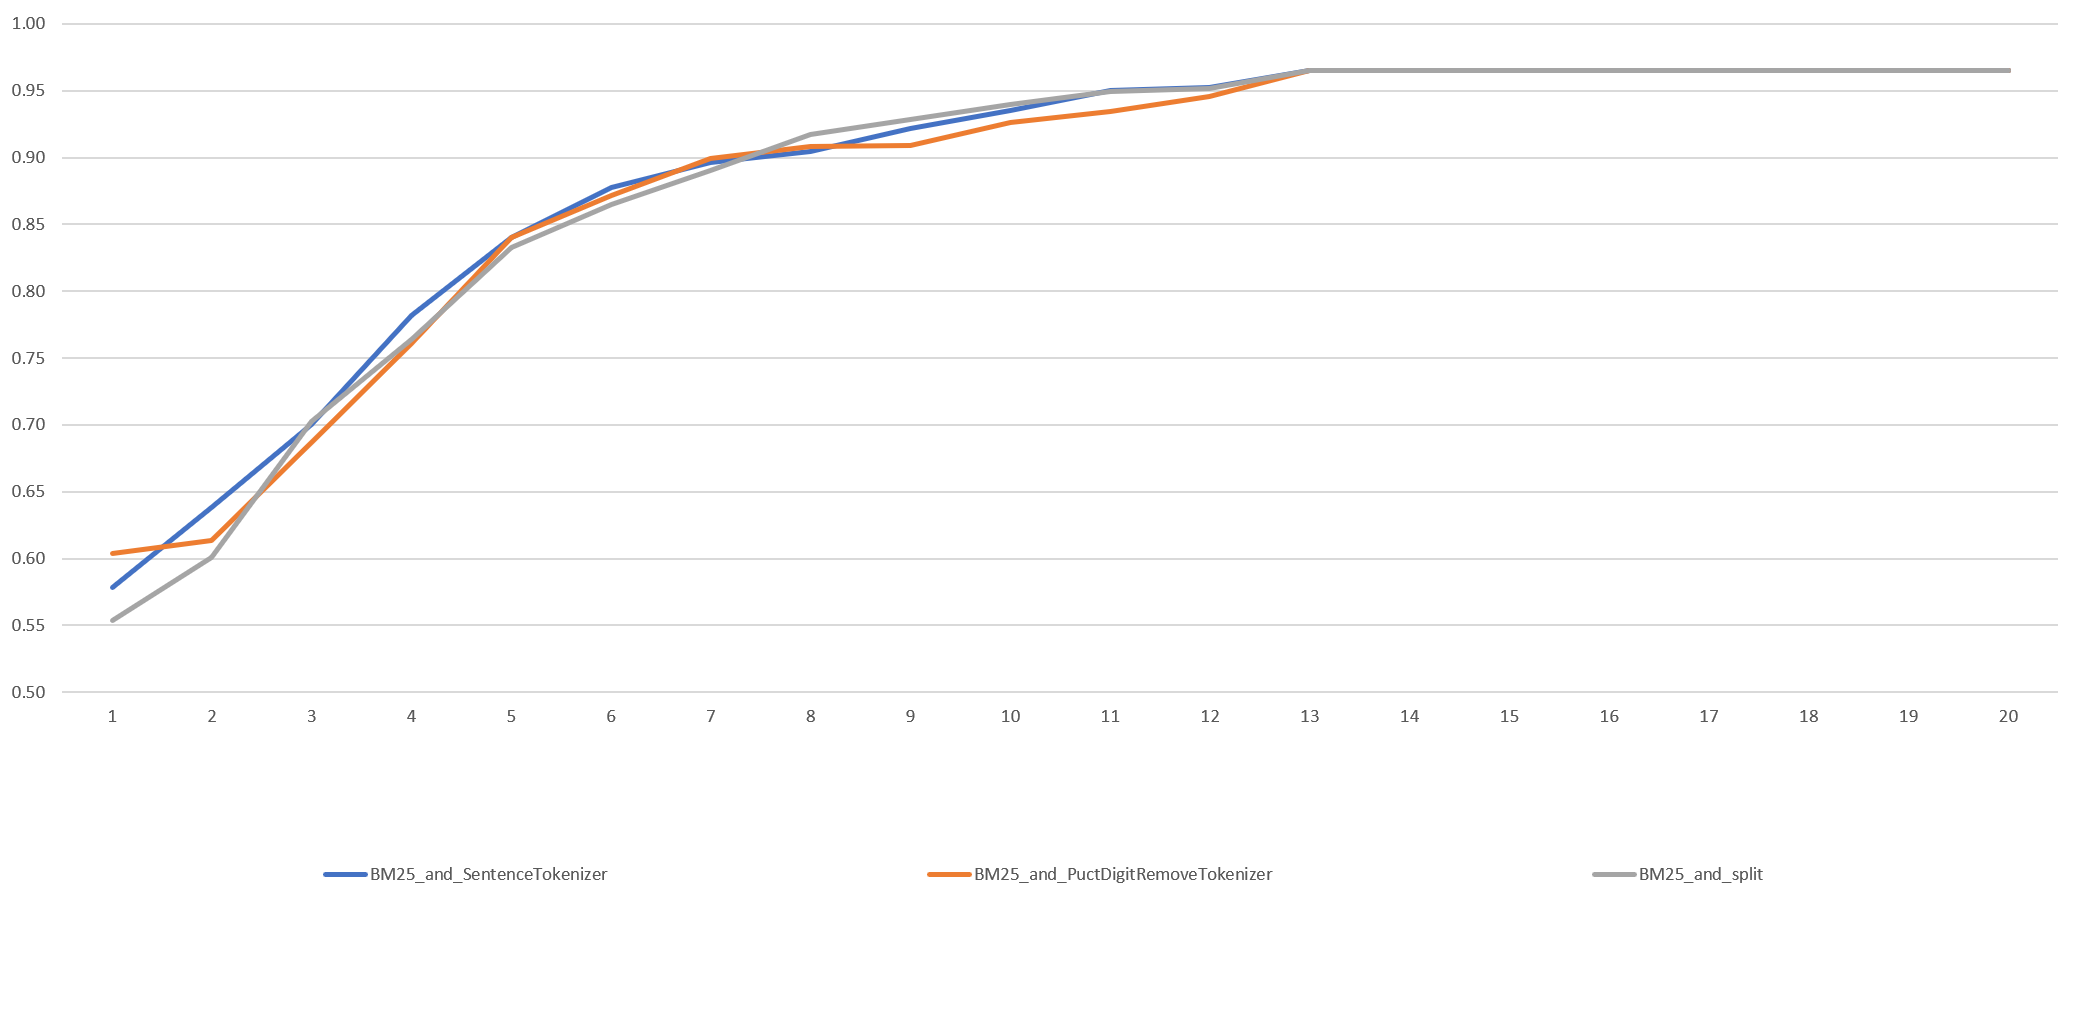
\includegraphics[width=\textwidth]{figure/partB_pairing_tokenizor_and.png}
						\caption{}
						\label{fig: pairingtokenizoreffect_and}
					\end{subfigure}
					\hfill
					\caption[]{Effect of tokenizor. (a)FastBM25 with "or" filter with different tokenizors. (b) BM25 with "and" filter with different tokenizors.}
					\label{fig: pairingtokenizoreffect}
				\end{figure}
			
			\paragraph{Keyword filtering} % or>and / tokenizor no big effect / more keywords better prediction
			
				\textbf{The Boolean logic filter function} ("and" filter and "or" filter) has no effect on non-hybrid models.
				By comparing the Bert Hybrid model performance, model with "or" filter function, its' performance is categorized as "middle M@L score", model with "and" filter is categorized as "low M@L score". Similar tendency is also discovered in other hybrid models. It can be concluded that hybrid model using "or" logic filter has better performance compared with hybrid model with "and" filter.
				
				\textbf{Tokenizers} (SentenceTokenizer,  PuctDigitRemoveTokenizer, split) used for filtering the keywords is found has no big effect in influencing the models behavior as can be seen from figure \ref{fig: pairingtokenizoreffect}.					
				
			
		\subsubsection{Retrieving Task}
			In the retrieving task, different retrieval models are applied concluding concluding BM25, FastBM25, Sent2Vec, BERT and their hybrid versions.
			A human rating score {0,1,2,3,4} is given to each retrieved search result according to its relevance to the query, quantitative metrics like ROUGE and NDCG are used for retrieval performance evaluation.
			
			The retrieving performance of all the models using different metrics are normalized to the range of [0,1] and collected together as shown in figure \ref{fig: partbnormalizedevaluationmetrics_all}.
			
			\begin{figure}[htbp]
				\centering
				\begin{subfigure}[b]{1\textwidth}
					\centering
					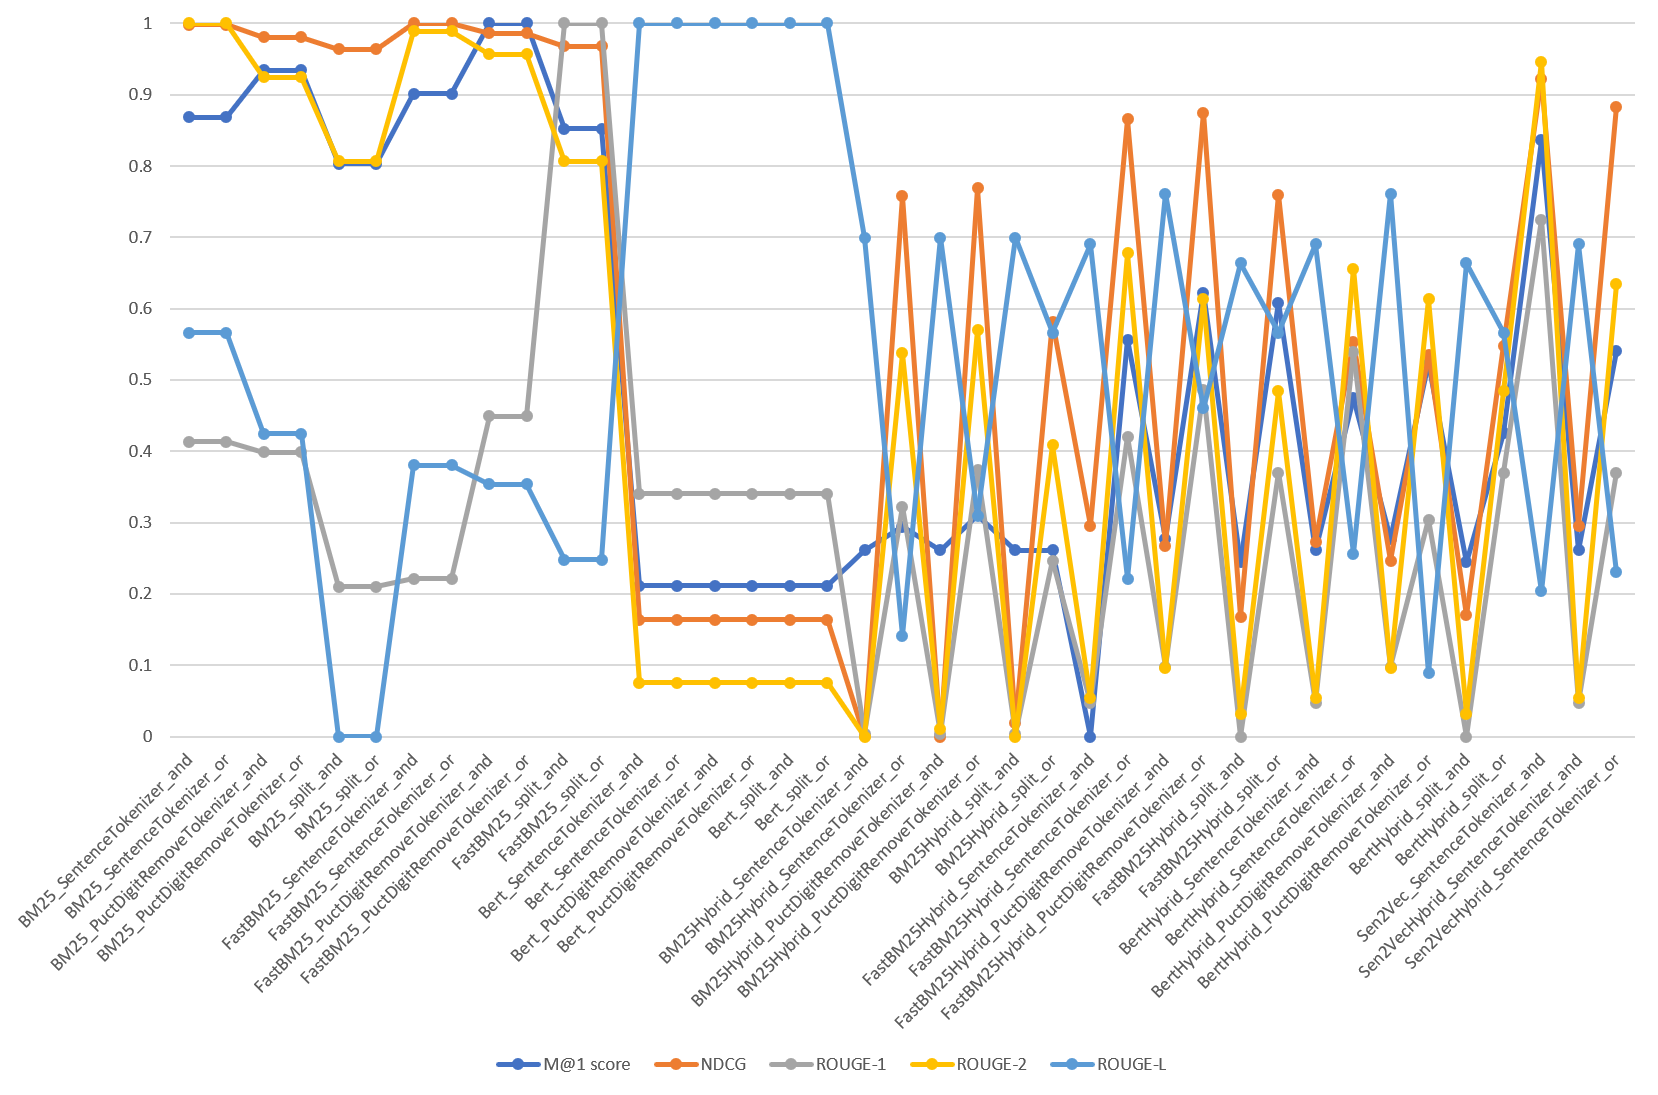
\includegraphics[width=\textwidth]{figure/partB_normalized_evaluation_metrics.png}
					\caption{}
					\label{fig: partbnormalizedevaluationmetrics_all}
				\end{subfigure}
				\hfill
				\begin{subfigure}[b]{1\textwidth}
					\centering
					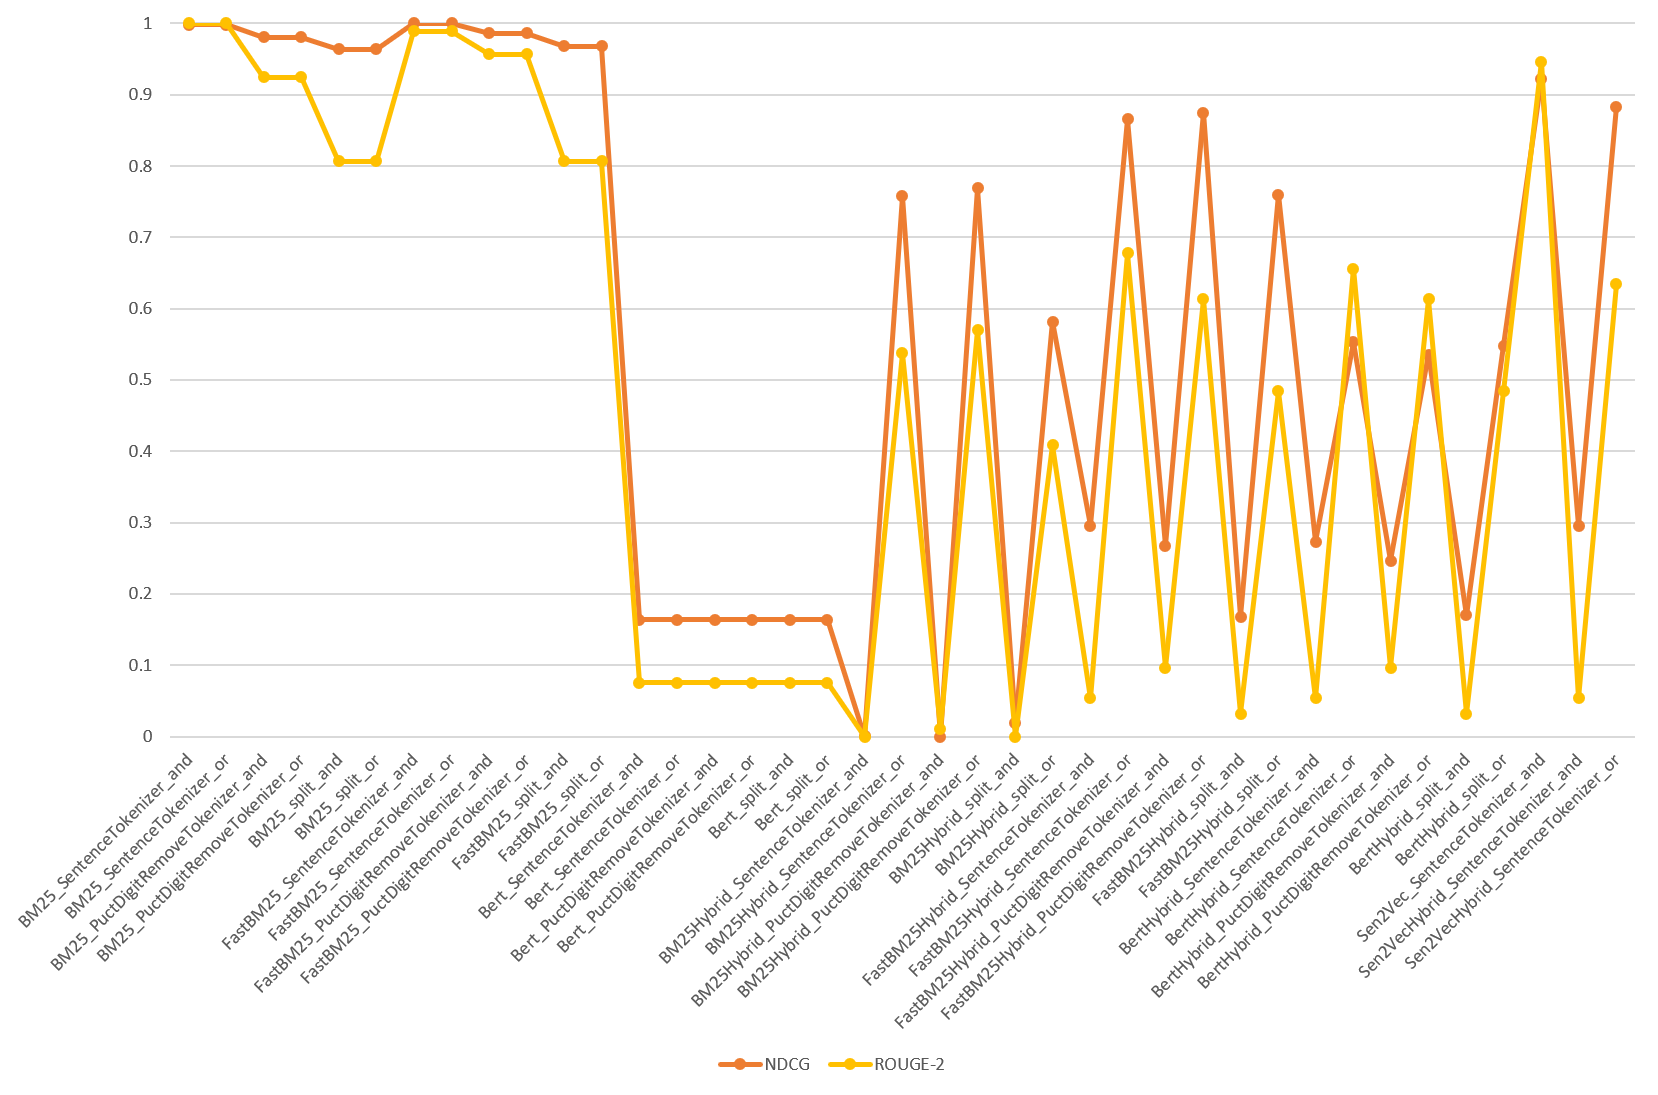
\includegraphics[width=\textwidth]{figure/partB_normalized_evaluation_metrics_part.png}
					\caption{}
					\label{fig: partbnormalizedevaluationmetrics_part}
				\end{subfigure}
				\hfill
				\caption[]{Normalized scores of different evaluation matrices using different models in retrieving task.(a) all the metrics. (b) NDCG and ROUGE-2 metrics.}
				\label{fig: partB_normalized_evaluation_metrics}
			\end{figure}
			
			
			\paragraph{Evaluation metrics comparison}
			
				M@L score is not used for retrieving evaluation and is used for pairing task, the M@1 score in the figure is shown as a reference which helps indicate the tendency of model performance.
				
				By checking the score tendency of different models in the figure, it seems that ROUGE-2 and NDCG score tend to reveal the performance of different models compared with other evaluation metrics.
				
				As shown in figure \ref{fig: partbnormalizedevaluationmetrics_part}, the ROUGE-2 score and NDCG is extracted from all the metrics.
				It can be found that NDCG scores are tend to have higher normalized values compared with ROUGE-2 value, which indicates that NDCG can be a metric which can reveal the model performance better compared with other matrices.
				
			\paragraph{Retrieval methods comparison}
				
				As shown in left side of the figure \ref{fig: partbnormalizedevaluationmetrics_all} (or figure \ref{fig: partbnormalizedevaluationmetrics_part}), the BM25 and FastBM25 model have higher normalized values than other models which indicates BM25 and FastBM25 model have the best retrieving performance in "Retrieval Task". Adding hybrid functions seems to have bad influence to the task performance. In addition BERT model seem to have the worst performance compared with other methods.
				
			\paragraph{Keyword selection comparison}
			
				\textbf{The Boolean logic} have obvious influence on hybrid models. As shown in the right side of figure \ref{fig: partbnormalizedevaluationmetrics_part}, with an "and" logic, the model performance is much worse than the "or" logic hybrid version.
				
				\textbf{Tokenizors function} can also influence the performance, although the influence is not big, a tendency that models with SentenceTokenizer and  PuctDigitRemoveTokenizer seem to have a higher normalized performance scores than models with split function.
				
	\subsection{Conclusion}
		\subsubsection{Pairing task}
		
			With the pairing task M@L results and the evaluation, it can be concluded that:
			\begin{itemize}
				\item BM25 and FastBM25 models have best retrieving performance compared with other models. Considering the computing speed, FastBM25 can be a more preferred model compared with BM25 model which requires shorter computation time and similar retrieving performance.
				\item Boolean logic filter has no effect on non-hybrid models and hybrid model with "or" logic has better performance compared with hybrid model with "and" filter.
				\item The tokenizors' effect on performance is not obvious on pairing task.
				\item Higher number of keywords is supposed to lead to a better prediction performance.
			\end{itemize}
		
		\subsubsection{Retrieval tasks}
		
			With the retrieval task results and evaluation, it can be concluded that:
			\begin{itemize}
				\item Both ROUGE-2 and NDCG metrics can well reveal the retrieval methods performance, and NDCG metric is found can indicate model performance better than ROUGE-2 metric.
				\item BM25 and FastBM25 models have best retrieving performance compared with other methods. Considering the computing speed, FastBM25 can be a more preferred model compared with BM25 model.
				\item For hybrid models, "or" Boolean logic can have a better retrieving performance compared with "and" Boolean logic.
				\item Tokenizors like "SentenceTokenizer" and "PuctDigitRemoveTokenizer" have a better performance compare with "split" function.
			\end{itemize}
			
			
			
			
			
		
\chapter{Summary}

\chapter{Appendix} \label{sk: dataandcode}
	

	\section{Dataset Introduction} 	
	
	\begin{figure}[htbp]
		\centering
		\begin{subfigure}[b]{0.48\textwidth}
			\centering
			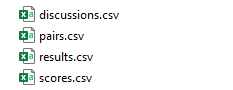
\includegraphics[width=\textwidth]{figure/dataset_structure}
			\caption{}
			\label{fig: datasetstructure}
		\end{subfigure}
		\hfill
		\begin{subfigure}[b]{0.48\textwidth}
			\centering
			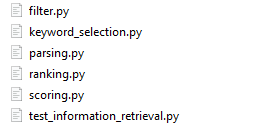
\includegraphics[width=\textwidth]{figure/code_structure}
			\caption{}
			\label{fig: codestructure}
		\end{subfigure}
		\hfill
		\caption[]{(a) Prepared dataset structure. (b) Code module structure.}
		\label{fig: structures}
	\end{figure}
	
	There are four parts of the dataset as shown in figure \ref{fig: datasetstructure} : 
	\begin{itemize}
		\item \textbf{discussions} contains document ids, discussion ids, and text of discussions,
		\item \textbf{results} contains document ids, result ids, and text of results, 
		\item \textbf{pairs}  contains document ids, discussion ids, and result ids, 
		\item \textbf{scores}  contains document ids of result paragraphs, result ids, document ids of discussion paragraphs, discussion ids, scores.			
	\end{itemize}				
	
	An example of the dataset created for scoring the result paragraphs and discussion paragraphs ("scores" part of the dataset) is shown in table \ref{tab: result_discussion_score}.
	
	\begin{table}[htbp]
		\centering
		\begin{tabular}{rrrrr}
			\toprule
			\multicolumn{1}{l}{doc\_id\_result} & \multicolumn{1}{l}{result\_id} & \multicolumn{1}{l}{doc\_id\_discussion} & \multicolumn{1}{l}{discussion\_id} & \multicolumn{1}{l}{score} \\
			\midrule
			1421389 & 0     & 1421389 & 0     & 4 \\
			1421389 & 0     & 1421389 & 3     & 2 \\
			653044 & 1     & 653044 & 2     & 4 \\
			2442696 & 1     & 2442696 & 1     & 2 \\
			2442696 & 1     & 193334 & 5     & 0 \\
			363993 & 1     & 363993 & 1     & 4 \\
			363993 & 1     & 363993 & 2     & 2 \\
			360628 & 1     & 363993 & 1     & 1 \\
			363993 & 1     & 995302 & 2     & 2 \\
			\midrule
			&       &       &       &  \\
		\end{tabular}%
		\caption{An example of the result and discussion scores.}
		\label{tab: result_discussion_score}%
	\end{table}%
	
	For each paper, an id to every result paragraph and discussion paragraph is given, and these result and discussion paragraphs are manually scored, i.e. pair result paragraphs to discussion paragraphs. 
	For example, if discussion paragraph 0 discusses result paragraphs 0 and 1, then we have 2 pairs {0,0} {0,1} for the paper. 
	Then we manually give a score {0,1,2,3,4} to some random discussion-result pairs from a subset of 100 papers. 
	
	\section{Code Module Introduction}	% code introduction
	
	As shown in figure \ref{fig: codestructure} 5 modules have been created in this search engine system :
	\begin{itemize}
		\item \textbf{parsing module} contains some functions to read and pre-process dataset,
		\item \textbf{keyword\_selection module} helps to build keyword scorer which score tokens in a query to generate keywords and then to build keyword selector based on scorer, 
		\item \textbf{filter module} helps to build a corpus filter which fetches an id list of documents based on specific filter strategy (AND, OR), 
		\item \textbf{ranking module} builds a ranker based on models like BM25, BERT, Sen2vec model, etc. and their hybrid versions, 
		\item \textbf{test\_information\_retrieval} module evaluates a prediction based on M-score, ROUGE score, DCG score, etc., it provides an easy way to test the whole system.     		
	\end{itemize}
	Table \ref{parsing} to \ref{test} show details in these modules.
	
	\begin{table}[htbp] 			
		\caption{\label{parsing}parsing} 
		\resizebox{\textwidth}{!}{
			\begin{tabular}{ll} 
				\toprule 
				name & description  \\ 
				\midrule 
				parse\_exemple\_file& Load exemple file. \\ 
				get\_dataset & Create example dataset from loaded dataframe.  \\ 
				get\_part2\_datasets & Load part2 dataset.\\ 
				SentenceTokenizer & Tokenizer removing all characters which are not from the set [0-9A-Za-z].\\
				PuctDigitRemoveTokenizer & Tokenizer removing all the punctuations.\\
				get\_ngrams & Get n-grams.\\
				add\_unigram & Add unigram into inverted index according to new document.\\
				get\_doc\_id\_mapping & Get index-to-id mapper and id-to-index mapper.\\
				get\_inverted\_index\_data & Compute inverted index, return a dictionary.	\\	
				\bottomrule 
		\end{tabular} }
	\end{table}
	
	\begin{table}[htbp] 
		\caption{\label{keywordselection}keyword\_selection} 
		\resizebox{\textwidth}{!}{
			\begin{tabular}{ll} 
				\toprule 
				name & description  \\ 
				\midrule 
				get\_unique\_token\_occurrences & Get occurrences of each token,return a map from tokens to frequencies in the input. \\ 
				add\_doc\_unigrams & Add unigram into inverted index. \\ 
				InvertedIndex & Wrapper to help work with the inverted index.  \\
				KeywordScorer & Abstract class to score tokens in a query to generate keywords.\\
				TfidfKeywordScorer & Scorer based on tf-idf metric.\\
				KeywordSelector &  Abstract class to select keywords based on scores generated by a scorer.\\
				SelectKKeywordSelector & Simple strategy that select a fixed number of keywords taken by decreasing score.\\
				\bottomrule 
		\end{tabular} }
	\end{table}
	
	\begin{table}[htbp] 
		\caption{\label{filter}filter} 
		\resizebox{\textwidth}{!}{
			\begin{tabular}{ll} 
				\toprule 
				name & description  \\ 
				\midrule 
				FilterStrategy & Interface of the corpus filter based on the results of the keyword selection. \\ 
				AndFilterStrategy & Implementation of filter strategy that take the intersection of the documents. \\ 
				OrFilterStrategy & Implementation of filter strategy that take the union of the documents.  \\
				CorpusFilter & Corpus filter that uses strategies injected in the init method to personalize how the filtering is done.\\
				CorpusFilterBuilder & Corpus filter builder that build a filter based on filter strategy, keyword scorer, and keyword selector.\\
				
				\bottomrule 
		\end{tabular} }
	\end{table}
	
	\begin{table}[htbp] 
		\caption{\label{ranking}ranking} 
		\resizebox{\textwidth}{!}{
			\begin{tabular}{ll} 
				\toprule 
				name & description  \\ 
				\midrule 
				Ranker & Abstract class that rank documents based on a given query.\\ 
				Bm25Ranker & Ranker based on the BM25 model.\\ 
				FastBM25Ranker &  Ranker based on the FastBM25 model. \\
				EmbeddingRanker & Ranker based on the Embedding model.\\
				Sent2VecRanker &  Ranker based on Sen2vec model.\\
				BertRanker & Rnker based on BERT model.\\
				HybridRanker & Abstract Hybrid ranker.\\
				Bm25HybridRanker & Hybrid version of the ranker based on the BM25 model.\\
				FastBm25HybridRanker & Hybrid version of the ranker based on the FastBM25 model.\\
				EmbeddingHybridRanker & Hybrid version of the ranker based on the Embedding model.\\
				\bottomrule 
		\end{tabular} }
	\end{table}
	
	\begin{table}[htbp] 
		\caption{\label{test}test\_information\_retrieval} 
		\resizebox{\textwidth}{!}{
			\begin{tabular}{ll} 
				\toprule 
				name & description  \\ 
				\midrule 
				get\_tokenizer\_fn & Get tokenizer. \\ 
				get\_corpus\_filter & Get corpus filter.  \\ 
				get\_ranker & Get ranker.  \\ 
				test\_pairing & Evaluation of prediction based on M-score.\\
				test\_retrieval & Evaluation of prediction based on ROUGE score and DCG score. \\
				
				\bottomrule 
		\end{tabular} }
	\end{table}
	

\end{document}
